\documentclass[10pt]{article}
\usepackage[a4paper, margin=1.5cm]{geometry}
\usepackage{mathptmx}
\usepackage[T1]{fontenc}
\usepackage{tikz}
\usetikzlibrary{positioning,arrows.meta,shapes.geometric,fit,backgrounds,calc}
\usepackage{caption}
\captionsetup{font=small, labelfont=bf, skip=4pt}
\pagestyle{empty}

\definecolor{jsonkey}{RGB}{163,21,21}
\definecolor{jsonnumber}{RGB}{9,134,88}
\newcommand{\fld}[1]{{\footnotesize #1}}
\newcommand{\newfld}[1]{{\footnotesize\bfseries\color{jsonnumber}#1}}

\begin{document}

% single-column-width preview (\columnwidth simulated at ~85mm)
\begin{figure}[t]
  \centering
  \resizebox{85mm}{!}{%
  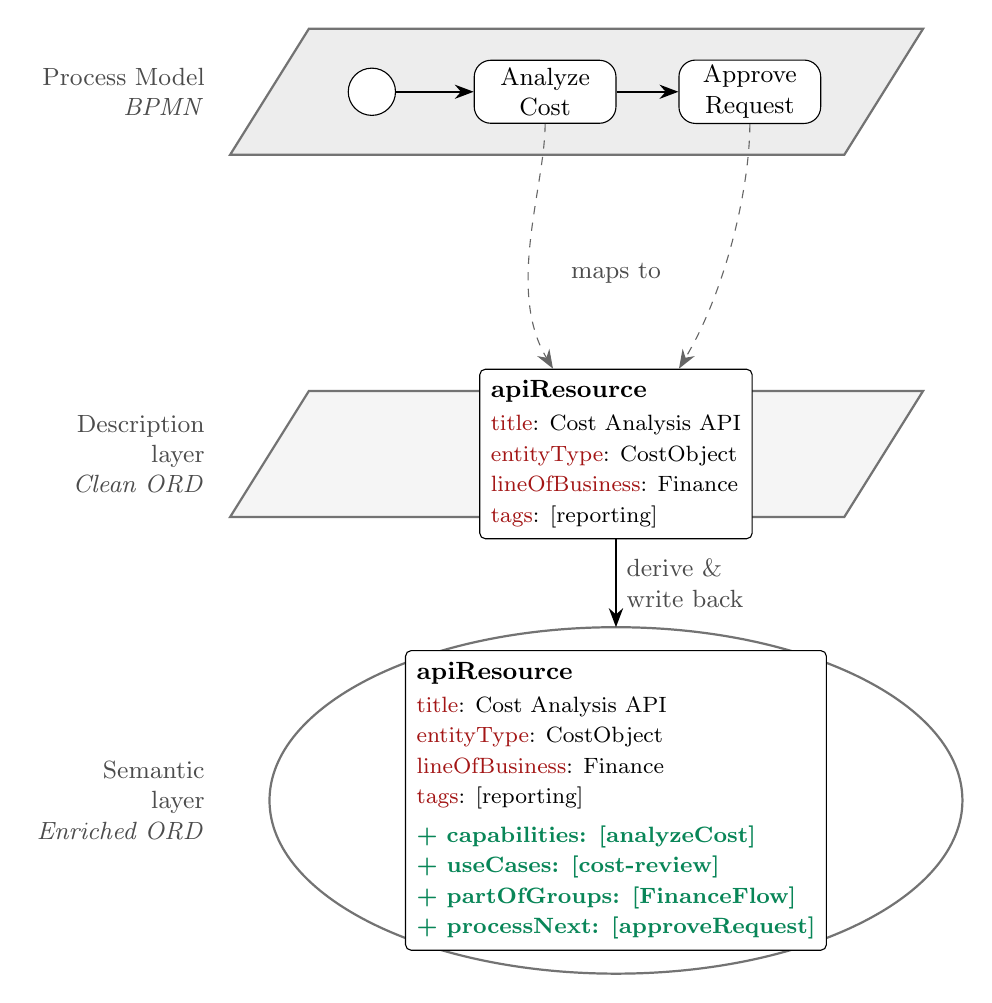
\begin{tikzpicture}[
    plane/.style={draw=black!55, thick},
    res/.style={draw, rounded corners=2pt, align=left, inner sep=4pt, fill=white,
                font=\small},
    act/.style={draw, rounded corners=6pt, minimum width=18mm, minimum height=8mm,
                align=center, inner sep=2pt, fill=white, font=\small},
    ev/.style={draw, circle, minimum size=6mm, inner sep=0pt, fill=white, font=\scriptsize},
    arr/.style={-{Stealth[length=2.4mm]}, semithick},
    maparr/.style={-{Stealth[length=2.4mm]}, dashed, black!60},
    lbl/.style={font=\small, black!70}
  ]

  % ================= META LEVEL PLANE (Process Model) =================
  \fill[black!7]  (6mm,104mm) -- (84mm,104mm) -- (94mm,120mm) -- (16mm,120mm) -- cycle;
  \draw[plane]    (6mm,104mm) -- (84mm,104mm) -- (94mm,120mm) -- (16mm,120mm) -- cycle;
  \node[lbl, anchor=east, align=right] at (4mm, 112mm) {Process Model\\\textit{BPMN}};

  \node[ev]  (start) at (24mm, 112mm) {};
  \node[act] (a1)    at (46mm, 112mm) {Analyze\\Cost};
  \node[act] (a2)    at (72mm, 112mm) {Approve\\Request};
  \draw[arr] (start) -- (a1);
  \draw[arr] (a1) -- (a2);

  % ================= DESCRIPTION LAYER (Clean ORD) =================
  \fill[black!4]  (6mm,58mm) -- (84mm,58mm) -- (94mm,74mm) -- (16mm,74mm) -- cycle;
  \draw[plane]    (6mm,58mm) -- (84mm,58mm) -- (94mm,74mm) -- (16mm,74mm) -- cycle;
  \node[lbl, anchor=east, align=right] at (4mm, 66mm) {Description\\layer\\\textit{Clean ORD}};

  \node[res] (clean) at (55mm, 66mm) {%
    \textbf{\small apiResource}\\[1pt]
    \fld{\textcolor{jsonkey}{title}: Cost Analysis API}\\
    \fld{\textcolor{jsonkey}{entityType}: CostObject}\\
    \fld{\textcolor{jsonkey}{lineOfBusiness}: Finance}\\
    \fld{\textcolor{jsonkey}{tags}: [reporting]}%
  };

  % mapping arrows: activity -> clean ORD resource
  \draw[maparr] (a1.south) .. controls +(0,-8mm) and +(-6mm,10mm) .. ([xshift=-8mm]clean.north);
  \draw[maparr] (a2.south) .. controls +(0,-8mm) and +(6mm,10mm)  .. ([xshift=8mm]clean.north);
  \node[lbl, fill=white, inner sep=1pt] at (55mm, 89mm) {maps to};

  % ================= SEMANTIC LAYER (Enriched ORD) =================
  \node[res, anchor=center] (enr) at (55mm, 22mm) {%
    \textbf{\small apiResource}\\[1pt]
    \fld{\textcolor{jsonkey}{title}: Cost Analysis API}\\
    \fld{\textcolor{jsonkey}{entityType}: CostObject}\\
    \fld{\textcolor{jsonkey}{lineOfBusiness}: Finance}\\
    \fld{\textcolor{jsonkey}{tags}: [reporting]}\\[3pt]
    \newfld{+ capabilities: [analyzeCost]}\\
    \newfld{+ useCases: [cost-review]}\\
    \newfld{+ partOfGroups: [FinanceFlow]}\\
    \newfld{+ processNext: [approveRequest]}%
  };
  \begin{scope}[on background layer]
    \draw[plane] (enr.center) ellipse (44mm and 22mm);
  \end{scope}
  \node[lbl, anchor=east, align=right] at (4mm, 22mm) {Semantic\\layer\\\textit{Enriched ORD}};

  % derive arrow: clean (description) -> enriched (semantic), downward
  \draw[arr, line width=1pt] (clean.south) -- (55mm, 44mm)
    node[midway, right, lbl, align=left] {derive \&\\write back};

  \end{tikzpicture}}%
  \caption{Process-driven semantic enrichment of ORD. A process model (meta level) is mapped onto Clean-ORD resources in the description layer; the mapping deterministically derives four typed fields (\texttt{capabilities}, \texttt{useCases}, \texttt{partOfGroups}, \texttt{processNext}) that are written back into the resource, producing its Enriched-ORD state in the semantic layer. The resource identity is preserved; only the semantic layer is added.}
  \label{fig:enrichment-preview}
\end{figure}

\end{document}
